\documentclass[12pt]{article}
\usepackage{multicol} %multicolumns
\usepackage{siunitx} %log table stuff
\usepackage{flafter}
\usepackage{amsmath} %math stuff
\usepackage{amssymb} %math symbols
\usepackage{graphicx} %including photos
\usepackage{wrapfig} %for wrapping figure
%\graphicspath{{./Report For Titanium Doping/}} %path of folder from where photo needs to be extracted, NOT NECESSARY AT ALL TIMES
\usepackage[utf8]{inputenc}
\usepackage{float} %Using [H] command to stop picturefloating around
\usepackage{enumerate} %changing labels of lists
\usepackage{fancyhdr}
\usepackage{dsfont} %for set notations and other fancy letters
\usepackage{mathrsfs}
\usepackage[compat=1.0.0]{tikz-feynman}

\usepackage{geometry}
\geometry{
a4paper,
total={170mm,257mm},
top=20mm,
}
\usepackage{array}
\setlength\extrarowheight{4pt}
%\usepackage[dvipsnames]{xcolor} %for using coloured text
\usepackage{longtable,pdflscape,booktabs} % long table stuff
\usepackage{lscape} 
\usepackage{caption}
\captionsetup{labelformat=empty}
\captionsetup[subfigure]{labelformat=empty}
\usepackage{subcaption}
\usepackage{setspace} %for desired spacing between lines
\usepackage{blindtext} % for blind text in contents page
\usepackage[normalem]{ulem} %dash and dotted underline
\usepackage{bm} % for bold math symbols- using command \boldsymbol
\usepackage{mathtools} %for rcases
\usepackage{hyperref} %for hyperlinks
\usepackage{romannum} %for Roman Numerals
\usepackage[makeroom]{cancel} % for striked out or other stuff in math environment
\usepackage{tikz}
\usepackage{empheq} %  fancy math stuff
\usepackage{xfrac}
\usepackage{fancybox} %for fancy boxes
\usepackage{circuitikz}
\usepackage{listings}

\allowdisplaybreaks
\colorlet{linkequation}{blue} %making coloured equation refernces

\usetikzlibrary{shadows} %defines shadows
\usepackage[framemethod=tikz]{mdframed}
\usepackage{tcolorbox} %coloured boxes

\tikzset{rndblock/.style={rounded corners,rectangle,draw,outer sep=1pt,inner sep=5pt,line width=1pt}}

% Command Definition
% 1 optional to customize the aspect, 2 mandatory: text to be framed
\newcommand{\mybox}[2][]{\tikz[baseline=(h.base)]\node[rndblock,#1] (h) {#2};}

%definining new command to make coloured equation references
\newcommand*{\myref}[1]{%
  \begingroup
    \hypersetup{
      linkcolor=linkequation,
      linkbordercolor=linkequation,
    }%
    \ref{#1}%
  \endgroup
}

%Setting equations a particular colour
\hypersetup{
colorlinks=true,
linkcolor=black,
filecolor=magenta,
urlcolor=blue,
citecolor=blue,
}

\parskip 1ex

%For circled numbers
\newcommand*\circled[1]{\tikz[baseline=(char.base)]{
            \node[shape=circle,draw,inner sep=2pt] (char) {#1};}}
            
%command for making capital roman numerals
\newcommand{\RomanNum}[1]{\MakeUppercase{\romannumeral #1}}


%%%%%%%%%%%%%%%%%%%%%%%%%%%%%%%%%%%%%%%%%%%%%%%%%%%%%%%%%%%%%%%%%%%%%%%%%%%%%%%%%%%%%%%%%%%%%%%%%%%%%%%%%%%%%%%%%%%%%%%%%%%%%%%%%%%%%%%%%%%%%%%%%%%%%%%%%%%%%%%%%%%%%%%%%%%%%%%%%%%%%%%%%%%%% DOCUMENT BEGINS %%%%%%%%%%%%%%%%%%%%%%%%%%%%%%%%%%


%\pagestyle{fancy}
%\fancyhf{}
%\fancyhead[LO]{\rightmark}
%\fancyhead[RE]{\leftmark}

\usepackage{titlesec, blindtext}
\titleformat{\section}[hang]{\Huge\bfseries}{\Roman{section}. \hspace{20pt}}{0pt}{\Huge\bfseries}

\titleformat*{\subsection}{\Large\bfseries}
\titleformat*{\subsubsection}{\large\bfseries}

\usepackage{tocloft}
\renewcommand{\cftsecleader}{\cftdotfill{\cftdotsep}}
\renewcommand{\cftsecaftersnum}{.}%

%%%%%%%%%%%%%%%%%%%%%%%%%%%%%%%%%%%%%%%%
\definecolor{codegreen}{rgb}{0,0.6,0}
\definecolor{codegray}{rgb}{0.5,0.5,0.5}
\definecolor{codepurple}{rgb}{0.58,0,0.82}
\definecolor{backcolour}{rgb}{0.95,0.95,0.92}

\lstdefinestyle{mystyle}{
    backgroundcolor=\color{backcolour},   
    commentstyle=\color{codegreen},
    keywordstyle=\color{magenta},
    numberstyle=\tiny\color{codegray},
    stringstyle=\color{codepurple},
    basicstyle=\ttfamily\footnotesize,
    breakatwhitespace=false,         
    breaklines=true,                 
    captionpos=b,                    
    keepspaces=true,                 
    numbers=left,                    
    numbersep=5pt,                  
    showspaces=false,                
    showstringspaces=false,
    showtabs=false,                  
    tabsize=2
}

\lstset{style=mystyle}
%%%%%%%%%%%%%%%%%%%%%%%%%%%%%%%%%%%%%%%%%%%%%%%%%%

\begin{document}
\doublespace
%making the title page
\pagenumbering{gobble}
\begin{titlepage}
	\begin{center}
		\vspace*{0.2cm}
		\textbf{\uline{P441/P442 - Open Lab Experiment}} \linebreak
		\vspace{1.5cm}\linebreak
		\textbf{\Large{Antenna Simulation for 21cm Hydrogen Line}}\linebreak
		\vspace{2cm} \linebreak
		\textit{Submitted By} \linebreak \textbf{ASHMITA PANDA} \linebreak 
		\textbf{ROLL NO. 1811042} \linebreak
		School of Physical Sciences \linebreak National Institute of Science, Education and Research (NISER), Bhubaneswar \linebreak
		Date of Submission : 
		\vspace{2.5cm} \linebreak
		\textit{Under the Guidance of} \linebreak \textbf{Dr. Pratap Kumar Sahoo} \linebreak Associate Professor \linebreak School of Physical Sciences \linebreak National Institute of Science Education and Research (NISER), Bhubaneswar
		\vspace{1cm} \linebreak

	\end{center}
	\begin{figure}[H]
		\centering
		
\includegraphics[width=0.17\textwidth]{niser logo}
	\end{figure}
\end{titlepage}

\raggedright
\newpage
\pagenumbering{roman}

\singlespacing
%Table of Contents
\tableofcontents
\addtocontents{toc}{~ \hfill \textbf{Page} \par}
\onehalfspacing

\newpage
\pagenumbering{arabic}
\begin{center}
	\doublespacing
	\textbf{\Large Abstract} \linebreak
	21cm Hydrogen line is one of the most useful tool of Radio Astronomy in current times. It can give us information about galaxy structures and rotation curves. It also finds applications in cosmology to probe the period from recombination to reionisation. \linebreak
  In this report, an attempt has been made to design an antenna for detecting this 21cm line. First, the theory of waveguides and antennas has been discussed. The optimum parameters have been calculated using ewa library in Matlab/Octave. The final design has been implemented using the software FEKO. 
\end{center}
\rule{17cm}{1pt}
%%%%%%%%%%%%%%%%%%%%%%%%%%%%%%%%%%%%%%%%%%%%%%%%%%%%%%%%%%%
%section - Introduction
\section{Introduction}
Antennas are one of the most widely used instrumental tool in physics. They are devices which either convert voltage from a transmitter to radio waves, or pick up radio waves from the atmosphere and convert it into voltage which can be detected by a receiver. \linebreak

In this this report, we aim to :
\begin{enumerate}[i.)]
  \item discuss the importance of the 21cm line in modern astronomy and cosmology
  \item discuss the theory of waveguides
  \item discuss properties of antennas
  \item design the antenna using FEKO 
\end{enumerate} 
%%%%%%%%%%%%%%%%%%%%%%%%%%%%%%%%%%%%%%%%%%%%%%%%%%%%%%%%%%%
%section - 21CM HYDROGEN LINE
\section{21cm Hydrogen Line}
%subsection - Theory
\subsection{Theory}
Neutral hydrogen is the most abundant element of the Universe. It is made up of one proton and one electron. 
Both the proton and electron are spin-1/2 particles. They can either be in up-spin or down-spin orientation. \linebreak

At any given point of time, the electron and proton in the neutral hydrogen atom, can either be aligned parallel to each other, or anti-parallel to each other. 
\begin{figure}[H]
  \centering
  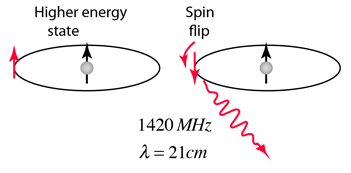
\includegraphics[width=0.5\textwidth]{Images/hflip.png}
  \caption{Fig 1. Two orientations of Neutral Hydrogen}
  \caption{\tiny Source : \url{http://hyperphysics.phy-astr.gsu.edu/hbase/quantum/h21.html}}
\end{figure}

The parallel spin state is the higher energy state compared to the anti-parallel spin state. The energy difference between the states is around 5.874eV. \linebreak

Whenever a neutral hydrogen atom goes from the parallel spin state to the anti-parallel spin state, it releases this energy in the form of a photon. This transition is called the the Spin-flip transition. \linebreak

From the Einstein-Planck equation :
\begin{equation}
  E=h \nu \label{eq:1}
\end{equation}
We can find the frequency of the emitted photon as 1420MHz. This corresponds to a wavelength of $\lambda=21$cm. 
%subsection - Importance
\subsection{Importance}
\subsubsection{In Radio Astronomy} % subsubsection 1
The 21cm line falls in the radio frequency range. It can easily penetrate the interstellar clouds and the Earth's atmosphere, thus can be observed without much interference. \linebreak

If we assume hydrogen atoms to be uniformly distributed throughout the galaxies, we should observe the 21cm line from all directions. The waves we receive will either be redshifted or blueshifted to different extents, depending on the location of their emission in the galaxy. \linebreak

We can then use this information to measure the rotation curve of our galaxy and the relative speed of each spiral arm. This information could in turn be used to indirectly calculate the mass of the galaxy. 
\begin{figure}[H]
  \centering
  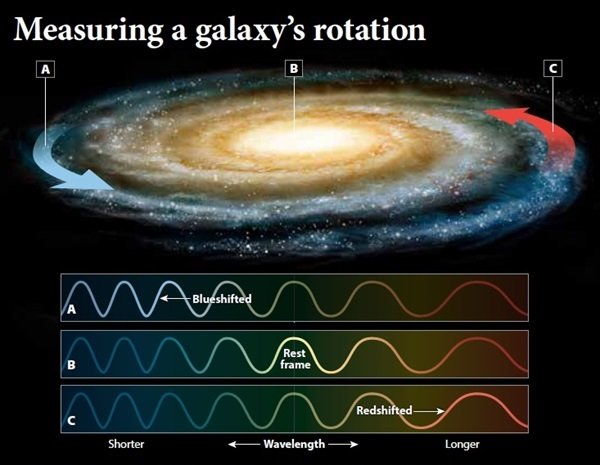
\includegraphics[width=0.5\textwidth,height=0.2\textheight]{Images/GalaxyRotation.jpg}
  \caption{Fig 2. Rotation Curve of a Galaxy}
  \caption{\tiny Source : \url{https://physicsopenlab.org/2020/09/08/measurement-of-the-milky-way-rotation/}}
\end{figure}
\subsubsection{In Cosmology} %subsubsection 2
The 21cm hydrogen line could be used in cosmology to probe the ``dark ages'' of the Universe, i.e., the period from recombination to reionisation. \linebreak
The hydrogen line from that epoch is highly red-shifted and obtained in the frequency range of 200MHz to 9MHz on Earth. \linebreak

We can obtain a picture of how the reionisation occured via this information, as we should obtain holes in the 21cm background spectrum from that epoch which correspond to hydrogen atoms which got ionised by the radiation from stars or quasars.
%%%%%%%%%%%%%%%%%%%%%%%%%%%%%%%%%%%%%%%%%%%%%%%%%%%%%%%%%%%%%section - WAVEGUIDES
\section{Waveguides}
Before building an antenna, we need to first talk about waveguiding structures. 
%subsection - What Are Waveguides?
\subsection{What Are Waveguides?}
Waveguides are structures which can guide waves, like sound waves or electromagnetic waves in a particular direction with minimal loss in energies. \linebreak

Waveguides for electromagnetic waves are made up of hollow metallic (conducting) tubes. They can carry high frequency radio waves. \linebreak

They can be of several types, namely circular, rectangular, elliptical, ridged etc. 
\begin{figure}[H]
  \centering
  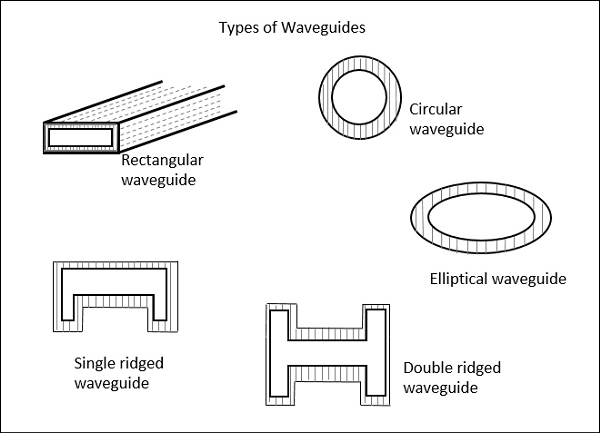
\includegraphics[width=0.5\textwidth]{Images/types_of_waveguides.jpg}
  \caption{Fig 3. Types of Waveguides}
  \caption{\tiny Source : \url{https://www.tutorialspoint.com/microwave_engineering/microwave_engineering_waveguides.htm}}
\end{figure}
%subsection - Arbitrary Waveguide
\subsection{Arbitrary Waveguide}
Let us consider a waveguide with some arbitrary cross section.
\begin{figure}[H]
  \centering
  \includegraphics[width=0.4\textwidth]{Images/arbitrary_waveguide.jpg}
  \caption{Fig 4. Arbitrary Waveguide Structure}
\end{figure}
Let's consider z to be the longitudinal direction, and x-y to be the transverse directions. Writing the EM waves :
\begin{align*}
  \vec{E}&=\vec{E}_{\perp}+E_z \hat{z} \, , \qquad \vec{E}_{\perp}=E_x \hat{x}+E_y \hat{y} \\
  \vec{H}&= \vec{H}_{\perp} + H_z \hat{z} \, , \qquad \vec{H}_{\perp} = H_x \hat{x}+H_y \hat{y} 
\end{align*}
We know from Maxwell's equation :
\begin{equation}
  \nabla \times \vec{E} = -j\omega \mu \vec{H} \label{eq:2}
\end{equation}
where, $\mu$ is the permeability of the space. \linebreak
Using the forms of EM waves written above :
\begin{align*}
  & \left( \nabla_{\perp}+\dfrac{\partial}{\partial z} \hat{z} \right) \times \left( \vec{E}_{\perp}+E_z \hat{z} \right) = -j\omega \mu \left( \vec{H}_{\perp}+ H_z \hat{z} \right) \\
  \implies & \nabla_{\perp} \times E_{\perp} + \nabla_{\perp}\times \left( E_z \hat{z} \right) +\dfrac{\partial}{\partial z}\hat{z}\times \vec{E}_{\perp} + \cancelto{0}{\dfrac{\partial}{\partial z} \hat{z}\times \left( E_z \hat{z}\right)} = -j\omega \mu \left( \vec{H}_{\perp}+H_z \hat{z}\right)
\end{align*}
The last term on LHS goes to zero as it involves the cross product of two parallel vectors. \linebreak
We can also see that the first term on LHS is along z direction, and the second and third terms are transverse terms. Equating the transverse components we obtain :
\begin{equation}
  \vec{H}_{\perp}=-\dfrac{1}{j\omega \mu} \left\{ \nabla_{\perp} \times \left( E_z \hat{z} \right) + \dfrac{\partial}{\partial z} \hat{z}\times \vec{E}_{\perp} \right\} \label{eq:3}
\end{equation}
Similarly, using the other Maxwell's equation :
\begin{equation}
  \nabla \times \vec{H} = j\omega \varepsilon \vec{E} \label{eq:4}
\end{equation}
where, $\epsilon$ is the permittivity of the space. \linebreak
We obtain the transverse component of electric field as :
\begin{equation}
  \vec{E}_{\perp} = \dfrac{1}{j\omega \varepsilon} \left\{ \nabla_{\perp}\times \left( H_z \hat{z} \right)+\dfrac{\partial}{\partial z}\hat{z}\times \vec{H}_{\perp} \right\} \label{eq:5}
\end{equation}
Now substituting for $\vec{H}_{\perp}$ from (\myref{eq:3}) in (\myref{eq:5}) :
\begin{equation*}
  \omega^2 \mu \varepsilon - \dfrac{\partial}{\partial z} \hat{z}\times \dfrac{\partial}{\partial z} \hat{z} \times \vec{E}_{\perp} = -j\omega \mu \nabla_{\perp} \times \left( H_z \hat{z} \right)+\left( \dfrac{\partial}{\partial z}\hat{z} \right) \times \nabla_{\perp} \times \left( E_z \hat{z} \right)
\end{equation*}
Using the triple product identity :
\begin{equation*}
  \vec{A}\times \vec{B}\times \vec{C}=\left( \vec{A}.\vec{C} \right)\vec{B}-\left( \vec{A}.\vec{B} \right)\vec{C}
\end{equation*}
We simplify the triple product terms in the equation above :
\begin{align*}
  \dfrac{\partial}{\partial z}\hat{z}\times \dfrac{\partial}{\partial z} \hat{z} \times \vec{E}_{\perp} &= - \dfrac{\partial^2}{\partial z^2}\vec{E}_{\perp} \\
  \dfrac{\partial}{\partial z}\hat{z}\times \nabla_{\perp}\times E_z \hat{z} &= \nabla_{\perp} \left( \dfrac{\partial E_z}{\partial z} \right)
\end{align*}
The final equation now becomes :
\begin{equation}
  \omega^2 \mu \varepsilon \vec{E}_{\perp} +\dfrac{\partial^2}{\partial z^2}\vec{E}_{\perp} = -j\omega \mu \nabla_{\perp}\times \left( H_z \hat{z} \right)+\nabla_{\perp} \left( \dfrac{\partial E_z}{\partial z} \right) \label{eq:6}
\end{equation}
The Maxwell's equations have only two independent components. Thus, we can choose the z-component of the electric and magnetic fields as the two independent components. So, (\myref{eq:6}) gives us how the transverse electric field depend on the independent components $E_z$ and $H_z$. \linebreak

Taking a travelling wave antasz along the z direction :
\begin{equation}
  E\, , H \sim \exp(-\gamma z) \label{eq:7}
\end{equation}
$\gamma$ is called the absorption coefficient. \linebreak

We ignore solutions for waves travelling in negative direction after reflection by assuming the waveguide is of infinite length. \linebreak
Given the ansatz in (\myref{eq:7}), we can write :
\begin{equation*}
  \dfrac{\partial}{\partial z} \equiv -\gamma \, , \quad \dfrac{\partial^2}{\partial z^2} \equiv \gamma^2
\end{equation*}
Using this in (\myref{eq:6}) :
\begin{equation*}
  \left( \omega^2 \mu \varepsilon+\gamma^2 \right) \vec{E}_{\perp} = -j\omega \mu \nabla_{\perp} \times \left( H_z \hat{z} \right)-\gamma \nabla_{\perp} E_z
\end{equation*}
We can define :
\begin{equation}
  \omega^2\mu \varepsilon+\gamma^2 = h^2 \label{eq:8}
\end{equation}
$h$ is the propagation constant for the transverse wave. \linebreak

Using this, we get the final form for the transverse electric and magnetic fields as :
\begin{align}
  \vec{E}_{\perp} &= -\dfrac{j \omega \mu}{h^2} \nabla_{\perp} \times \left( H_z \hat{z} \right) - \dfrac{\gamma}{h^2}\nabla_{\perp} E_z \label{eq:9}\\
  \vec{H}_{\perp} &= \dfrac{j\omega \varepsilon}{h^2}\nabla_{\perp} \times \left( E_z \hat{z} \right)-\dfrac{\gamma}{h^2} \nabla_{\perp} H_z \label{eq:10}
\end{align}
Since we have chosen the z-components of electric and magnetic fields as the independent components, we can find the complete solutions for the wave motion if we can determine $E_z$ and $H_z$. \linebreak

For a medium that is lossless, 
\begin{equation}
  \gamma = j \beta \label{eq:11}
\end{equation}
We can conclude that :
\begin{enumerate}[i.)]
  \item $E_z$ and $H_z$ both cannot be zero, unless h is zero. Converse is also true. This implies that if both the longitudinal components are zero, there is no transverse wave propagation in the waveguide. EM wave travels as if it is in free space. 
  \item The above mode is called the TEM mode, i.e., Transverse Electric and Magnetic field mode. It is a non-dispersive mode.
  \item When $E_z=0$ and $H_z \neq 0$, it is called the TE mode, i.e., the Transverse Electric mode. It is dispersive mode. 
  \item When $E_z \neq 0$ and $H_z=0$, it is called the TM mode, i.e., the Transverse Magnetic mode. It is a dispersive mode.
\end{enumerate}
%subsection - Rectangular Waveguides
\subsection{Rectangular Waveguides}
A rectangular waveguide is one of the most common types of waveguides used. 
\begin{figure}[H]
  \centering
  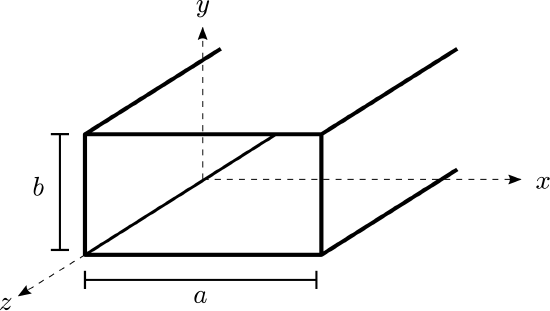
\includegraphics[width=0.5\textwidth]{Images/rectangular.png}
  \caption{Fig 5. Rectangular Waveguide}
  \caption{\tiny Source : \url{https://www.tutorialspoint.com/microwave_engineering/microwave_engineering_waveguides.htm}}
\end{figure}
Let us consider the electromagnetic waves moving along z-direction. \linebreak
We will also assume that for this structure $a\geq b$.\linebreak
\subsubsection{TM Mode} %subsubsection - TM Mode
We will first consider the solutions of TM Mode, i.e.,
\begin{equation*}
  E_z\neq 0 \, , \quad H_z=0
\end{equation*}
Writing the wave equation for electric field travelling in z-direction :
\begin{align*}
  & \nabla^2 E_z + \omega^2 \mu \varepsilon E_z =0 \\
  \implies & \dfrac{\partial^2 E_z}{\partial x^2}+\dfrac{\partial^2 E_z}{\partial y^2}+\dfrac{\partial^2 E_z}{\partial z^2}+\omega^2 \mu \varepsilon E_z=0 
\end{align*}
Applying separation of variables :
\begin{equation*}
  E_z(x,y,z) = X(x)Y(y)Z(z) 
\end{equation*}
Putting this in the wave equation, we obtain the final solution as :
\begin{align*}
  X(x)&= c_1 \cos(Ax)+c_2 \sin(Ax) \\
  Y(y)&= c_3 \cos(By)+c_4 \sin(By) \\
  Z(z)&= c_5 \exp(-j \beta z)+c_6 \exp(j \beta z)
\end{align*}
The solutions $X(x)$ and $Y(y)$ are standing wave solutions. The solution $Z(z)$ is the travelling wave solution.\linebreak

As we had assumed earlier that the waveguide we are using is of infinite length, and there is no reflected wave (wave travelling in -z direction), we can write $c_6=0$. \linebreak

Now using the four boundary conditions due to the four walls upon which $E_z$ is tangential, i.e.,
\begin{equation*}
  E_z = 0 \quad \text{ for } \quad x=0\, , \quad x=a \, , \quad y=0 \, , \quad y=a
\end{equation*}
we obtain the constants $A$ and $B$ as :
\begin{equation}
  A=\dfrac{m\pi}{a} \, , \quad B=\dfrac{n\pi}{b} \label{eq:12}
\end{equation}
We obtain the final solution for $E_z$ as :
\begin{equation}
  E_z = C \sin\left( \dfrac{m\pi}{a}x \right)\sin\left( \dfrac{n\pi}{b}y \right)\exp\left( -j\beta z \right) \label{eq:13}
\end{equation}
Now using the expression for $E_z$ (\myref{eq:13}) in (\myref{eq:9}) and (\myref{eq:10}), we obtain the transverse wave equations as :
\begin{align}
  E_x &= -\dfrac{j \beta}{h^2}\dfrac{\partial E_z}{\partial x} = -\dfrac{j \beta}{h^2}\left( \dfrac{m\pi}{a} \right) C \cos \left( \dfrac{m \pi x}{a} \right) \sin\left( \dfrac{n\pi y}{b} \right) \exp(-j\beta z) \label{eq:14} \\
  E_y &= -\dfrac{j \beta}{h^2}\dfrac{\partial E_z}{\partial y} = -\dfrac{j \beta}{h^2} \left( \dfrac{n\pi}{a} \right) C \sin\left( \dfrac{m\pi x}{a} \right)\cos\left( \dfrac{n\pi y}{b} \right) \exp(-j\beta z) \label{eq:15} \\
  H_x &= \dfrac{j\omega \varepsilon}{h^2} \dfrac{\partial E_z}{\partial y} = \dfrac{j \omega \varepsilon}{h^2}\left( \dfrac{n\pi}{b} \right) C\sin\left( \dfrac{m\pi x}{a} \right) \cos\left( \dfrac{n\pi y}{b} \right)\exp(-j\beta z) \label{eq:16} \\
  H_y &= -\dfrac{j\omega \varepsilon}{h^2} \dfrac{\partial E_z}{\partial x} = -\dfrac{j \omega \varepsilon}{h^2} \left( \dfrac{m\pi}{a} \right)C \cos\left( \dfrac{m\pi x}{a} \right)\sin\left( \dfrac{n\pi y}{b} \right) \exp(-j\beta z) \label{eq:17}
\end{align}
The conclusions we can immediately draw from the above equations are as follows :
\begin{enumerate}[i.)]
  \item The TM\textsubscript{00} mode does not exist. All the waves become zero. 
  \item If either $m=0$ or $n=0$, then also none of the components exist. Thus, TM\textsubscript{m0} and TM\textsubscript{0n} modes also do not exist.
  \item TM\textsubscript{11} is the lowest TM mode that can exist in the rectangular waveguide.
\end{enumerate}
Also, from (\myref{eq:8}), (\myref{eq:11}) and the separable solutions, we can write :
\begin{equation}
  h^2=\omega^2 \mu \varepsilon -\beta^2 = A^2+B^2 = \left( \dfrac{m\pi}{a} \right)^2 + \left( \dfrac{n \pi}{b} \right)^2 \label{eq:18}
\end{equation}
\subsubsection{TE Mode} %subsubsection - TE Mode
Now considering the TE Mode, i.e.,
\begin{equation*}
  E_z=0 \, , \quad H_z \neq 0
\end{equation*}
We need to first solve for $H_z$, as we did for the case of TM mode. \linebreak
After following the similar procedure, we obtain the form of $H_z$ as :
\begin{equation}
  H_z = C \cos\left( \dfrac{m\pi x}{a} \right)\cos\left( \dfrac{n\pi y}{a} \right) \exp(-j\beta z) \label{eq:19}
\end{equation}
We can analyse the above equation directly to look for possible lowest order modes.
\begin{enumerate}[i.)]
  \item For $m=n=0$, $H_z$ is a constant. It does not vary with time. So, all transverse components of the field is zero, i.e., $\vec{E}_{\perp}=\vec{H}_{\perp}=0$. This is because $\vec{E}_{\perp}$ and $\vec{H}_{\perp}$ contain space derivatives of $H_z$. From this we can immediately as $H_z$ must be zero too, as magnetic field cannot exist in the absence of a time-varying electric field. Thus, the TE\textsubscript{00} mode does not exist. 
  \item The TE\textsubscript{m0} and TE\textsubscript{0n} modes exist. Thus the lowest order mode could be either TE\textsubscript{10} or TE\textsubscript{01} mode.
\end{enumerate}
\subsubsection{Cut-off Frequency, Dominant Mode and Field Pattern}
We know from the preceding analysis that :
\begin{align*}
  h^2 &= \left( \dfrac{m\pi}{a} \right)^2 + \left( \dfrac{n \pi}{b} \right)^2 \\
  \beta^2 &= \omega^2 \mu \varepsilon - \left( \dfrac{m\pi}{a} \right)^2 - \left( \dfrac{n \pi}{b} \right)^2
\end{align*}
Now for a propagating wave, the frequency should be greater than some critical value for the term $\beta$ to be a real number. If $\beta$ is a complex number, it would mean the EM wave decays exponentially inside the waveguide. \linebreak

At the cut-off frequency of a mode, we have $\beta=0$. \linebreak
With this, we can find the equation for the cut-off frequency as follows :
\begin{equation}
  f_c = \dfrac{1}{2\pi \sqrt{\mu \varepsilon}} \left\{ \left( \dfrac{m\pi}{a} \right)^2+\left( \dfrac{n\pi}{b} \right)^2 \right\}^{1/2} \label{eq:20}
\end{equation}
From the above equation (\myref{eq:20}), we can calulate the cutoff frequencies of $TE_{10}$, $TE_{02}$ and $TM_{11}$ modes. We observe that :
\begin{equation*}
  f^c_{TE_{10}} < f^c_{TE_{01}} < f^c_{TM_{11}}
\end{equation*}
Thus, $TE_{10}$ mode is the lowest order mode of a rectangular waveguide. It has the minimum cutoff frequency. Consequently, it is also the dominant mode of the rectangular waveguide as the probability of a wave being in $TE_{10}$ mode is the greatest. It depends only on the `a' side of the waveguide. \linebreak

In the dominant $TE_{10}$ mode :
\begin{align*}
  H_z &= C \cos\left( \dfrac{\pi x}{a} \right)\exp(-j\beta z) \\
  E_y &= -\dfrac{j \omega \mu}{\left( \pi/a \right)^2}C \left( \dfrac{\pi}{a} \right)\sin\left( \dfrac{\pi x}{a} \right)\exp(-j\beta z) \\
  H_x &= - \dfrac{j \omega \varepsilon}{\left( \pi/a \right)^2}C\left( \dfrac{\pi}{a} \right)\sin\left( \dfrac{\pi x}{a} \right) \exp(-j\beta z) \\
  E_x &= 0 \, , \quad H_y =0
\end{align*}
The field pattern of electric and magnetic field inside the waveguide depends on which mode is it being operated on. \linebreak
In the $TE_{10}$ mode, magnetic flux lines appear as continuous loops, and electric field lines occur as sinusodial waves on the x-y plane, which become zero on the $y=0$ and $y=b$ walls.
\begin{figure}[H]
  \centering
  \includegraphics[width=0.6\textwidth]{Images/fieldpatterns.jpg}
  \caption{Fig 6. Field Patterns inside Rectangular Waveguide}
  \caption{\tiny Source : \url{http://www.engineeringdone.com/te-tm-modes/te-tm-modes/}}
\end{figure}
%%%%%%%%%%%%%%%%%%%%%%%%%%%%%%%%%%%%%%%%%%%%%%%%%%%%%%%%%%%%%\section -Antenna Parameters
\section{Antenna Parameters}
All kinds of antennas can be characterised or studied using certain parameters which have been summarised in this section. 
%subsection - bandwidth
\subsection{Bandwidth}
The bandwidth gives us the frequency range over which an antenna operates. All waveguides have a lower cutoff frequency, $\omega_c$. So for an antenna to function properly, the frequency of the wave must be greater than the cutoff frequency. For optimum transport, the frequency of the wave must in the range of $1.25 \omega_c$ to $1.9\omega_c$. If the frequency is greater than $1.25\omega_c$ then dispersion down the waveguide gets minimised, and if the frequency is lesser than $1.9\omega_c$, then the higher order modes gets suppressed. 
%subsection - radiation pattern
\subsection{Radiation Pattern}
The radiation pattern of an antenna gives us the power radiated by it as a function of $\theta$ and $\phi$, i.e., as a function of direction. \linebreak
We can classify antennas into three types based on their radiation patterns :
\begin{enumerate}[i.)]
  \item \textbf{Isotropic} : Antenna radiates same amount of radiation in all directions.
  \item \textbf{Omni-directional} : The antenna is isotropic in one plane.
  \item \textbf{Directional} : There is no symmetry is power radiation of the antenna. It is usually radiates power as a single peak in some direction.
\end{enumerate}
%subsection - Field Regions
\subsection{Field Regions}
The electromagnetic fields surrounding an antenna could be divided into three regions :
\begin{enumerate}[i.)]
  \item \textbf{Far Fields} : These are the fields in the region far away from the antenna. The electric and magnetic fields do not change shape with distance.
  \item \textbf{Reactive Near Fields} : These are the fields in the immediate vicinity of the antenna. The electric and magnetic fields are out of phase by 90 degrees.
  \item \textbf{Radiative Near Fields} : These are the fields in the region between far fields and reactive near fields.
\end{enumerate}
%subsection - Directivity
\subsection{Directivity}
Directivity of an antenna is fundamental parameter. It gives us a measure of how directional the radiation pattern of an antenna is. \linebreak 
An antenna which radiates equally in all directions, i.e., the isotropic antenna, would have zero directivity.\linebreak

If we write the normalised field pattern of an antenna is written in spherical harmonics as $F(\theta, \phi)$, then the mathematical formula for directivity is given as :
\begin{equation}
  D = \left[ \dfrac{1}{4\pi}\int^{2\pi}_0 \int^{\pi}_0 |F(\theta, \phi)|^2 \sin\theta d\theta d\phi \right]^{-1}
\end{equation}
%subsection - Gain
\subsection{Gain}
The gain of the antenna measures how much power is radiated by the antenna in the peak directivity direction when compared to an isotropic source. \linebreak
It takes into account the actual losses that might have occurred in the system. Thus, it is often used more to specify the characteristics of an antenna compared to directivity.
%subsection - Main Lobe, side lobe, Null and HPBW
\subsection{Lobes and HPBW}
\begin{figure}[H]
  \centering
  \includegraphics[width=0.5\textwidth]{Images/radiation-lobes-of-antenna.jpg}
  \caption{Fig 7. Radiation Pattern of an Antenna}
\end{figure}
\paragraph{Main Lobe} : It is the region around the direction of peak radiation of the antenna, usually the region within 3dB of the peak gain.
\paragraph{Side Lobes} : These are the smaller beams away from the main beam. These are usually the radiation along undesired directions. 
\paragraph{Null} : These are the regions along which no power is radiated. 
\paragraph{HPBW} : Half Power Full Bandwidth is the angular separation in which the power radiated by the antenna decreases by 50\% of the maximum power radiated in the peak direction.
%%%%%%%%%%%%%%%%%%%%%%%%%%%%%%%%%%%%%%%%%%%%%%%%%%%%%%%%%%%%%section - Horn antenna
\section{Horn Antenna}
Horn Antenna is one of the most commonly used antenna structures. It consists of a rectangular waveguide which flares out at one end. They are directional antennas. we power the waveguide using a quarter wavelength monopole antenna. \linebreak

The flare is needed to prevent a sudden change of impedance. If the waveguide is open-ended and has no flare, the change in impedance will be too high and a part of the wave energy will get reflected back into the waveguide. \linebreak 

Thus, the flare essentially acts as a transitional structure. It ensures the impedance of the waveguide matches with the impedance of the free space, and the radiation can flow smoothly. \linebreak

Based on the shape of the flare, the horn antennas can be classified into three types.
\begin{enumerate}[i.)]
  \item \textbf{H-Plane sectoral} : The `a' side (longer side) is flared and `b' side (shorter side) is flat.
  \item \textbf{E-Plane sectoral} : The `b' side (shorter side) is flared and `a' side (longer side) is flat.
  \item \textbf{Pyramidal} : Both `a' and `b' sides are flared.
\end{enumerate}
\begin{figure}[H]
  \centering
  \includegraphics[width=0.8\textwidth]{Images/typesofhornantenna.png}
  \caption{Fig 8. Types of Horn Antenna}
  \caption{\tiny Source : \url{https://www.ece.rutgers.edu/~orfanidi/ewa/ch21.pdf}}
\end{figure}
%subsection - Pyramidal Horn antenna
\subsection{Pyramidal Horn Antenna}
We have used a pyramidal horn antenna for our setup. \linebreak
Let A and B be length of the sides of the horn. We can look at the geometry of the horn to determine certain parameters.
\begin{figure}[H]
  \centering
  \includegraphics[width=0.6\textwidth]{Images/hornantennageometry.png}
  \caption{Fig 9. Geometry of Pyramidal Horn Antenna}
  \caption{\tiny Source : \url{https://www.ece.rutgers.edu/~orfanidi/ewa/ch21.pdf}}
\end{figure}
$R_A$ and $R_B$ are the perpendicular distance between the plane of the waveguide opening and the plane of the horn. They must be equal in length. They are given as :
\begin{equation}
  R_a = \dfrac{A}{A-a}R_A \, , \quad R_b \dfrac{B}{B-b}R_B \label{eq:22}
\end{equation}
$\Delta_a$ and $\Delta_b$ represent the maximum deviation of the radial distance from the plane of the horn. Fpr any distance x along A and y along B, they are given as :
\begin{equation}
  \Delta_a(x)=\dfrac{x^2}{R_a} \, , \quad \Delta_b(y)=\dfrac{y^2}{R_b} \label{eq:23}
\end{equation}
%subsection - Determining Optimum parameters
\subsection{Determing Optimum Parameters}
If we wish to find the optimum dimensions of the flare, we need to define two parameters, $\sigma_a$ and $\sigma_b$. 
\begin{equation}
  \sigma^2_a = \dfrac{A}{2\lambda R_a} \, , \quad \sigma^2_b = \dfrac{B}{2\lambda R_b} \label{eq:24}
\end{equation}
Different values of $\sigma_a$ and $\sigma_b$ give us the corresponding flare parameters. Now, when we use these values along with the dimension of the waveguide and required gain, we can obtain the flare dimensions. \linebreak
These values are calculated using \textit{hopt} function in the ewa library in Matlab/Octave.
\begin{equation*}
  [A, B , R, err]=hopt[G,a,b,\sigma_a,\sigma_b,N]
\end{equation*}
where,
\begin{align*}
  G & \implies \text{Gain of the antenna} \\
  a,b & \implies \text{waveguide dimensions in units of wavelength} \\
  A,B & \implies \text{sides of the horn returned in units of wavelength}\\
  R & \implies \text{axial length from waveguide end to plane of horn given in units of wavelength}
\end{align*}
%%%%%%%%%%%%%%%%%%%%%%%%%%%%%%%%%%%%%%%%%%%%%%%%%%%%%%%%%%%%%section - construction
\section{Construction of Horn Antenna}
The construction of the horn antenna has been done in two steps. First, the optimum parameters of the flare were obatined using \textit{hopt} function of ewa libary in Octae/Matlab. Then, using the FEKO software the antenna was build and simulated for near and far fields. \linebreak
Two antennas have been designed
%subsection - antenna 1
\subsection{Antenna 1} %antenna 1
\subsubsection{Determing Flare Parameters from Octave/Matlab}
Since the frequency that we wish to detect is 1420MHz, for the first antenna, we chose the cutoff frequency $TE_{10}$ to be 1000MHz. It corresponded the cutoff wavelength of $\lambda_{c1}=30cm$. \linebreak
The side `a' was taken to be 15cm and side `b' was taken to 7.5cm. These are the most commonly used aspect ratios.
\begin{equation}
  a_1=\dfrac{\lambda_{c1}}{2}=15cm \, , \quad b_1=\dfrac{a_1}{2}=7.5cm \label{eq:25}
\end{equation}
The values of gain and sigma parameters were chosen to be :
\begin{equation}
  G=18dB\, , \quad \sigma_a=1.475 \, \quad \sigma_b=0.74 \label{eq:26}
\end{equation}
Using (\myref{eq:25}) and (\myref{eq:26}), the flare parameters are obtained as :
\begin{equation}
  A_1=0.96m \, , \quad B_1=0.484m \, , \quad R_1=0.861m \label{eq:27}
\end{equation}
\subsubsection{Contruction in FEKO}
A horn antenna with the parameters given in (\myref{eq:25}), (\myref{eq:26}) and (\myref{eq:27}) was constructed in CadFEKO. The near and far fields were simulated, and the results are shown below. 
\begin{figure}[H]
  \centering
  \includegraphics[width=0.6\textwidth]{Antenna 1/antenna.png}
  \caption{Fig 10. Antenna Gain for Far Field (3D plot)}
\end{figure}
\begin{figure}[H]
  \centering
  \includegraphics[width=0.6\textwidth]{Antenna 1/nearfield_perpendicular.png}
  \caption{Fig 11. Antenna Gain for Near Field (3D plot)}
\end{figure}
\begin{figure} [H]
  \begin{subfigure}[b]{0.6\textwidth}
      \centering
      \includegraphics[width=\textwidth]{Antenna 1/farfield_cartesian.png}
  \end{subfigure}%
  \begin{subfigure}[b]{0.65\textwidth}
      \centering
      \includegraphics[width=\textwidth]{Antenna 1/farfield_polar.png}
  \end{subfigure}
  \caption{Fig 12. Far Field Radiation Pattern in Cartesian and Polar Coordinates}
\end{figure}
%subsection - antenna 2
\subsection{Antenna 2}
\subsubsection{Determining Flare Parameters from Octave/Matlab}
In this case, the size of the antenna we attempted to reduce the size of the antenna. \linebreak
We chose the cutoff frequency $TE_{10}$ to be 1100MHz. It corresponded the cutoff wavelength of $\lambda_{c2}=27.2cm$. \linebreak
The side `a' was taken to be 13.6cm and side `b' was taken to 10cm. 
\begin{equation}
  a_2=\dfrac{\lambda_{c2}}{2}=13.6cm \, , \quad b_1=10cm \label{eq:28}
\end{equation}
The values of gain and sigma parameters were chosen to be :
\begin{equation}
  G=18dB\, , \quad \sigma_a=1.2593 \, \quad \sigma_b=1.0246 \label{eq:29}
\end{equation}
These are said to be the most optimal sigma parameter values. \linebreak
Using (\myref{eq:28}) and (\myref{eq:29}), the flare parameters are obtained as :
\begin{equation}
  A_1=0.749m \, , \quad B_1=0.604m \, , \quad R_1=0.69m \label{eq:30}
\end{equation}
\subsubsection{Contruction in FEKO}
A horn antenna with the parameters given in (\myref{eq:28}), (\myref{eq:29}) and (\myref{eq:30}) was constructed in CadFEKO. The near and far fields were simulated, and the results are shown below. 
\begin{figure}[H]
  \centering
  \includegraphics[width=\textwidth]{Antenna 2/antenna2.png}
  \caption{Fig 13. Antenna Gain for Far Field (3D plot)}
\end{figure}
\begin{figure}[H]
  \centering
  \includegraphics[width=0.8\textwidth]{Antenna 2/nearfield_2.png}
  \caption{Fig 14. Antenna Gain for Near Field (3D plot)}
\end{figure}
\begin{figure} [H]
  \begin{subfigure}[b]{0.6\textwidth}
      \centering
      \includegraphics[width=\textwidth]{Antenna 2/farfield_cartesian2.png}
  \end{subfigure}%
  \begin{subfigure}[b]{0.65\textwidth}
      \centering
      \includegraphics[width=\textwidth]{Antenna 2/farfield_polar2.png}
  \end{subfigure}
  \caption{Fig 15. Far Field Radiation Pattern in Cartesian and Polar Coordinates}
\end{figure}
%subsection -discussion
\subsection{Discussion}
We can see for both the antenna, that the radiation field is highly directive. We obtain a gain of upto 20dB. The size of the antenna is not extremely bulky and can be implemented physically. \linebreak
The near field simulated perpendicular to the aperture of the antenna highlights its directive nature. It shows very high gain in the direction of the horn.
%%%%%%%%%%%%%%%%%%%%%%%%%%%%%%%%%%%%%%%%%%%%%%%%%%%%%%%%%%%%%\section - Conclusion
\section{Conclusion}
In this report, we first discussed about the theory of waveguides and antenna parameters like directivity, bandwidth, gain, radiation pattern, etc. We also looked at the geometry of horn antennas and their various parameters. \linebreak

The optimal dimensions for the horn antenna were then calculated using Octave/Matlab, for given sigma parameters, gain and waveguide dimensions. The data from the same was used to contruct a horn antenna in FEKO and simulate near and far field patterns. \linebreak

Two antennas were designed by this process, both with gain 18dB. One was designed using the standard a/b ratio of 2, and the other was designed with $a/b=1.36$. In the second design, it was attempted to reduce the size of the antenna to make it less bulky without compromising the gain and directivity of the first design. \linebreak

We obtain both the antennas to be highly directive with gains of almost 20dB. Thus, the ratio $a/b=1.36$ allowed us to build a smaller antenna while keeping the gain at around 18-20dB. It can be considered as an improvement to the design.



\end{document}